\documentclass[11pt,a4paper]{article}
\usepackage[margin=2.2cm]{geometry}
\usepackage[T1]{fontenc}
\usepackage[utf8]{inputenc}
\usepackage{lmodern}
\usepackage{amsmath,amssymb}
\usepackage{booktabs}
\usepackage{enumitem}
\usepackage{xcolor}
\usepackage{tikz}
\usepackage{hyperref}
\hypersetup{colorlinks=true,linkcolor=blue!50!black,urlcolor=blue!50!black}
\setlist{itemsep=2pt,topsep=3pt}
\setlength{\parskip}{5pt}
\setlength{\parindent}{0pt}

\newcommand{\key}[1]{\textbf{#1}}
\newenvironment{qa}[1]{\par\medskip\textbf{Q: #1}\par\noindent\textbf{A:} }{\par}
\newcommand{\boxnote}[1]{\par\medskip\noindent\fcolorbox{black!40}{black!4}{\parbox{0.96\linewidth}{#1}}\par\medskip}

\title{RAP-FedWMMSE: the whole project in simple words\\[4pt]
\large A study guide for Group 12 (to understand the work and answer Sir)}
\author{Kushagra Kumar Arora, Chinmay Pramod Ardalkar, Rachit Yadav, Saurav Anand Jha}
\date{November 2026}

\begin{document}
\maketitle

\boxnote{\textbf{How to read this.} Section 1 is the story in one page. Sections 2--5 explain the ideas. Section 6
gives the results. Section 7 lists our weak points, honestly. Section 8 explains the Google Deep Review rounds.
Section 9 is a list of questions Sir might ask, with short answers. Section 10 says where everything is.}

\tableofcontents
\newpage

%=====================================================================
\section{The story in one page}

\textbf{The setting.} Imagine a city area with many small antennas (access points, \key{APs}) spread around,
instead of one big tower. All of them serve all the phones (\key{users}, or UEs) together. This is called
\key{cell-free massive MIMO}. It works well, except for one problem: if a building \emph{blocks} a user, every AP
near that user sees a very weak signal.

\textbf{The fix.} Put a few \key{relays} in the area. A relay is a small helper station. It listens to the APs,
understands (\emph{decodes}) the message, and then sends it again to the blocked user from a better position.

\textbf{The hard part.} Now we must decide many things together:
\begin{itemize}
  \item how every AP should point its signal (its \key{beam});
  \item how every relay should point its signal, and how it should listen;
  \item which relay helps which user (the \key{association});
  \item how to split time between ``APs talk'' and ``relays talk'' (the \key{phase split} $\tau$).
\end{itemize}
Doing this perfectly needs one central computer that knows every channel. That is slow and needs a lot of data
to be sent to the centre.

\textbf{Sir's idea: RAP-FedWMMSE.} Let every AP and relay solve its \emph{own} part, using only what it knows
locally plus a small amount of shared information. Each node runs a few steps of a well-known optimizer
(\key{WMMSE}). A small neural network tunes the step sizes of that optimizer. The nodes train their networks
with \key{federated learning}: they share model updates, not raw data. There is \key{no dataset}: the network
learns directly from the quantity we want to maximize.

\textbf{What we did.} We built the whole algorithm in Python, built every comparison method Sir asked for,
built an \emph{exact} solver that gives the true best possible answer on a tiny network, ran 14 experiments of
100 random user positions each, drew 14 graphs, wrote an IEEE paper, and improved it through two rounds of
Google Deep Review.

\textbf{What we found, in one line.} The method works well and fast for blocked users, but most of its gain
comes from the information sharing and from Steps 1--2 (choosing $\tau$ and relays), not from the neural
network; and federated learning gave no extra benefit in our setting. We report all of this honestly.

%=====================================================================
\section{Words you must know}

\begin{description}[style=nextline,leftmargin=1.2em]
\item[AP (access point)] A small base station with 2 antennas. We use 8 of them.
\item[UE (user equipment)] A phone. We use 8 users, each with 1 antenna.
\item[Relay] A helper station with 2 antennas. We use 2 relays. It is \emph{half-duplex}: it cannot listen and
  talk at the same time.
\item[Cell-free massive MIMO] Many APs serve all users together, with no ``cells''. Each user is served by its 4
  strongest APs (its \emph{cluster}).
\item[Channel / CSI] The ``path'' a signal takes from one antenna to another (how strong, what phase).
  \emph{CSI} = channel state information = knowing that path. \emph{Local CSI} = a node knows only its own paths.
\item[Blockage] An obstacle. A blocked user's direct signal from the APs is 25\,dB weaker (about 300 times).
  2 of our 8 users are blocked.
\item[Beam / beamforming] With several antennas, a node can ``aim'' its signal at one user and away from others.
  The beam is a small vector of complex numbers.
\item[Decode-and-forward (DF)] The relay first fully understands the message, then re-sends it. So a relayed
  user can only get as much data as the \emph{weaker} of the two hops. That is why the rate has a $\min$:
  rate $=\min(\text{what reaches the user},\ \text{what the relay can decode})$.
\item[Two phases and $\tau$] Each time slot is split. Phase I (fraction $\tau$ of the time): APs talk, users and
  relays listen. Phase II (fraction $1-\tau$): relays talk. $\tau$ is between 0.2 and 0.8.
\item[SINR] Signal-to-interference-plus-noise ratio: how strong my signal is compared to everything else.
  The data rate is about $\log_2(1+\text{SINR})$ bits per second per hertz.
\item[PF utility] Our main score: $\sum_k \ln(\text{rate}_k + 0.001)$. ``PF'' means \emph{proportional fair}.
  The logarithm punishes starving any user, so it rewards fairness. Higher is better. A negative value means
  some users get very low rates.
\item[Outage] A user is ``in outage'' if its rate is below a target, here $0.5$ bit/s/Hz.
\item[5th-percentile rate] The rate of the unluckiest 5\% of users. It tells how well we treat the weakest users.
\item[WMMSE] Weighted minimum mean-square error. A classic, trusted algorithm for designing beams. It repeats a
  simple update many times until the beams stop changing.
\item[Deep unfolding] Take an iterative algorithm (like WMMSE), keep only a few iterations (we use 6, called
  \emph{layers}), and let a neural network choose the step sizes of each layer. Fast, and still understandable.
\item[Federated learning (FL)] Several devices train models; they share only model \emph{updates} (not their
  data). \emph{FedAvg} is the basic version (everyone averages). \emph{Personalized} FL lets each node mix updates
  from similar nodes.
\item[Fronthaul] The cable that connects an AP to the network. It has limited capacity, so FL traffic must fit.
\item[MINLP and branch-and-bound] Our full problem has yes/no choices (which relay helps whom) and smooth choices
  (beams): a \emph{mixed-integer nonlinear program}. \emph{Spatial branch-and-bound} (we use the solver
  \emph{SCIP}) finds the true best answer, with a certificate, but only for tiny networks.
\item[Drop and deployment] A \emph{deployment} = where the APs and relays stand. A \emph{drop} = one random
  placement of the users. We use 10 deployments $\times$ 10 drops = 100 test cases.
\item[95\% confidence interval ($\pm$)] ``7.88 $\pm$ 0.51'' means: with 95\% confidence the true average is
  between 7.37 and 8.39. If two methods' difference has an interval that excludes 0, the difference is real.
\item[Paired comparison] Compare two methods on the \emph{same} drops, drop by drop. Much more precise than
  comparing two averages.
\end{description}

%=====================================================================
\section{The problem we solve}

For one time slot, choose: AP beams, relay beams, relay listening filters (\emph{combiners}), the relay--user
association, and $\tau$; so that the \textbf{PF utility is as large as possible}, while
\begin{itemize}
  \item every AP and relay stays within its power (1 watt each);
  \item each user gets at most 1 relay (we also test 2), and each relay helps at most 4 users;
  \item optionally, users should rarely fall below $0.5$ bit/s/Hz (QoS), and power use can be penalized
    (energy price $\lambda_E$).
\end{itemize}
This is called problem \textbf{P0} in the paper. It is hard (non-convex, with yes/no choices), so no fast method
is guaranteed to find the best answer.

\begin{center}
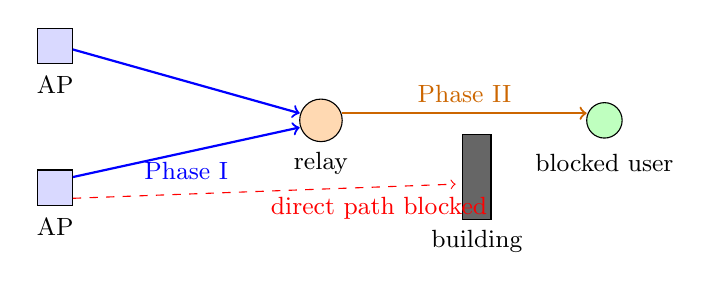
\begin{tikzpicture}[scale=0.9, every node/.style={font=\small}]
  \draw[fill=blue!15] (0,0) rectangle (0.5,0.5); \node at (0.25,-0.3) {AP};
  \draw[fill=blue!15] (0,2) rectangle (0.5,2.5); \node at (0.25,1.7) {AP};
  \draw[fill=orange!30] (4,1.2) circle (0.3); \node at (4,0.6) {relay};
  \draw[fill=green!25] (8,1.2) circle (0.25); \node at (8,0.6) {blocked user};
  \draw[fill=black!60] (6,-0.2) rectangle (6.4,1.0); \node at (6.2,-0.5) {building};
  \draw[->,thick,blue] (0.5,0.4) -- (3.7,1.1) node[midway,below] {Phase I};
  \draw[->,thick,blue] (0.5,2.2) -- (3.7,1.3);
  \draw[->,thick,orange!80!black] (4.3,1.3) -- (7.75,1.3) node[midway,above] {Phase II};
  \draw[->,dashed,red] (0.5,0.1) -- (5.9,0.3) node[pos=0.8,below] {direct path blocked};
\end{tikzpicture}
\end{center}

%=====================================================================
\section{Sir's algorithm, RAP-FedWMMSE, step by step}

The name means \emph{Role-Aware Personalized Federated WMMSE}. ``Role-aware'' = APs and relays have different
jobs, so they get different neural network front-ends. It works on two \key{timescales}:
\emph{slow} (once per ``epoch'', about once per second) and \emph{fast} (every time slot).

\subsection*{Slow timescale}
\begin{enumerate}[label=\textbf{Step \arabic*.},leftmargin=4em]
\item \textbf{Choose relays.} Give every (relay, user) pair a score: is the relay-to-user link stronger than the
  user's direct link? Is the APs-to-relay link strong? Is the relay disturbed by other APs? Is the user suffering
  (its QoS price)? Then pick the best pairs, respecting the limits, with an exact small optimization (a
  ``matching'').
\item \textbf{Choose $\tau$.} Try 61 values of $\tau$ between 0.2 and 0.8 and keep the best one for the
  measured signal strengths. In practice it usually picks 0.8 (the maximum): Phase I carries most of the data.
\item[\textbf{Step 3}] \textbf{Share a small summary ($\zeta_s$).} Every node receives 48 numbers: each user's
  ``suffering'' prices, the relay prices, how much interference each user measured, and last epoch's rates.
\end{enumerate}

\subsection*{Fast timescale (every time slot)}
\begin{enumerate}[label=\textbf{Step \arabic*.},leftmargin=4em,start=4]
\item \textbf{The neural network predicts settings.} Each node's small network looks at its own channels plus
  the 48-number summary and outputs: a step size and a ``damping'' for each of the 6 layers, a regularization
  value, and how to split its power among its users at the start.
\item[\textbf{Steps 5--8}] \textbf{Run 6 WMMSE layers.} In each layer: every node receives a shared message
  ($\zeta_f$, 352 numbers) describing how strongly every beam reaches every receiver; then each node improves its
  own beams with a WMMSE-type update, using its own channels plus that message; then it scales its beams back
  within its power limit. Special trick: with neutral settings, one layer is \emph{exactly} the classical WMMSE
  update. So the learning starts from a trusted algorithm and only adjusts it.
\item[\textbf{Step 9}] \textbf{Prices (primal--dual).} If a user stays below $0.5$ bit/s/Hz, its ``price'' goes up,
  so the next updates care more about it. If a relay hop is the bottleneck, that hop's price goes up.
\item[\textbf{Step 10}] \textbf{Robustness.} During training, we also test the beams on slightly wrong
  (``stale'') channels and penalize outage. The idea is that the model learns to be safe when channel knowledge
  is old. (In our tests, this part turned out to have no measurable effect; see Section 7.)
\end{enumerate}

\subsection*{Training and federated learning}
\begin{enumerate}[label=\textbf{Step \arabic*.},leftmargin=4em,start=11]
\item \textbf{Self-supervised training, no dataset.} Every epoch, new random users appear. The networks are
  trained to make the PF utility high. No labels, no stored dataset: the channels are simulated.
\item[\textbf{Step 12}] \textbf{Who wants to share?} A node becomes a candidate if its model changed a lot, its
  surroundings changed, it has not shared for a while, or its gradient is large.
\item[\textbf{Step 13}] \textbf{Who may share?} An exact ``knapsack'' picks the most urgent candidates within a
  40\,kB budget, and only if the node's fronthaul cable still has room after carrying user data.
\item[\textbf{Step 14}] \textbf{Compress.} Send only the largest 10\% of the update values (``top-$k$''), and
  remember the rest for next time (``error feedback'').
\item[\textbf{Step 15}] \textbf{Personalized mixing.} Each node mixes the received updates, giving more weight to
  nodes that are similar to it (similar position, load, role).
\end{enumerate}

\subsection*{Where we had to interpret Sir's text (ask Sir to confirm)}
\begin{enumerate}
\item \textbf{Step 9:} as written, the relay price could never go up (the formula was always $\le 0$). We used the
  difference ``destination rate minus relay-hop rate'', which is positive exactly when the relay is the bottleneck.
\item \textbf{Step 7:} instead of a plain gradient step, we used a regularized WMMSE step. It keeps Sir's learned
  step size, damping and regularization, and equals classical WMMSE with neutral settings. A plain gradient step
  performed much worse in our tests.
\item \textbf{Step 11:} in simulation, each node's gradient is computed through all nodes together. A real network
  would need an extra backward message exchange for this.
\item \textbf{Step 1:} the score weights ($1, 1, 0.25, 1$) and a ``relay must beat the direct link'' rule are our
  choices, tuned on deployments never used for testing.
\item \textbf{Training data:} fresh random users every epoch (with one fixed set of users, the model overfit).
\item \textbf{Fronthaul:} the cable limit restricts FL traffic only; user data is never cut.
\end{enumerate}

%=====================================================================
\section{What we compare against, and how we tested}

\subsection*{The methods}
\begin{itemize}
\item \textbf{Centralized WMMSE-SCA/AO} (Sir asked for it): one central computer knows everything and optimizes
  for up to 100 iterations. The strongest practical method; our ``gold standard''.
\item \textbf{Centralized WMMSE, no relay}: the same, but without relays, using the full time slot ($\tau=1$).
  Tells us what relays add.
\item \textbf{Local-WMMSE / No-FL} (Sir asked for it): each node optimizes alone, sharing nothing.
\item \textbf{RZF and MRT}: simple textbook beam rules with equal power.
\item \textbf{Ablations} (our own method with one part removed): with FedAvg instead of personalized FL; with no FL;
  the same layers \emph{untrained}; and (Round 2) untrained layers \emph{with} Steps 1--2, and undamped classical
  WMMSE.
\item \textbf{Exact MINLP} (Sir asked for it): SCIP branch-and-bound on a tiny network (2 APs, 1 relay, 2 users,
  1 antenna each). Gives a certified upper limit: no method can do better.
\end{itemize}

\subsection*{How we kept it fair}
\begin{itemize}
\item Every method is tested on the \emph{same} 100 drops and scored by the \emph{same} code.
\item Results are averages with 95\% confidence intervals; differences are paired drop by drop.
\item Training uses different random users than testing.
\item The no-relay method gets the whole time slot ($\tau = 1$). (An earlier version unfairly limited it; we fixed
  that even though it made our method look worse.)
\item Re-running gives identical numbers (we checked this several times).
\end{itemize}

\subsection*{The network (defaults)}
8 APs and 2 relays (2 antennas each), 8 users (1 antenna), 500\,m $\times$ 500\,m area, 20\,MHz, 1\,W per node,
city path-loss model (3GPP UMi), 2 of 8 users blocked by 25\,dB. Only 2 antennas per node, so that the central
and exact methods can still be solved.

\subsection*{The 14 graphs (one line each)}
\begin{tabular}{@{}ll@{}}
G01 & Distribution of user rates (who gets what). \\
G02 & Outage vs the target rate. \\
G03 & Average and worst-5\% rate vs transmit power. \\
G04 & PF utility vs number of users. \\
G05 & PF utility vs how many users are blocked. \\
G06 & PF utility vs number of relays (and 2 relays per user). \\
G07 & PF utility vs a fixed $\tau$. \\
G08 & PF utility vs how old/stale the channel knowledge is ($\rho$). \\
G09 & PF utility vs number of layers (trained vs untrained). \\
G10 & Distance from the certified best answer (tiny network). \\
G11 & Running time vs number of users. \\
G12 & Federated learning curves and data exchanged. \\
G13 & Utility vs power used (energy price $\lambda_E$). \\
G14 & Federated learning under a limited fronthaul cable. \\
\end{tabular}

%=====================================================================
\section{The results}

\subsection*{Main table (default network, 100 drops)}
\begin{center}
\small
\begin{tabular}{lcccc}
\toprule
Method & PF utility & Mean rate & Worst 5\% rate & Time per drop \\
\midrule
Centralized WMMSE & $9.88 \pm 0.40$ & 4.57 & 0.67 & 5.05 s \\
Centralized, no relay & $9.80 \pm 0.53$ & 5.41 & 0.18 & 1.46 s \\
\textbf{RAP-FedWMMSE (ours)} & $\mathbf{7.88 \pm 0.51}$ & \textbf{3.49} & \textbf{0.57} & \textbf{0.16 s} \\
Same layers, untrained & $3.87 \pm 0.46$ & 2.06 & 0.36 & 0.03 s \\
Local-WMMSE & $-3.43 \pm 0.43$ & 0.89 & 0.20 & 0.32 s \\
RZF / MRT & $-2.43$ / $-5.60$ & 1.13 / 0.58 & 0.20 / 0.20 & $\le$0.001 s \\
\bottomrule
\end{tabular}
\end{center}
(Rates in bit/s/Hz. Outage at $0.5$: centralized 3.0\%, ours 4.0\%, no relay 10.9\%.)

\subsection*{What is good}
\begin{itemize}
\item \textbf{Best method without a central computer}: $+11.3$ PF utility over Local-WMMSE (wins on all 100 drops).
\item \textbf{76\%} of the centralized method's average rate, with almost the same outage (4.0\% vs 3.0\%).
\item \textbf{Relays protect weak users}: the worst-5\% rate is $0.57$ with our method vs $0.18$ without relays
  (about 3 times better).
\item \textbf{Fast}: 0.16\,s per drop vs 5\,s for centralized (about 30 times less computation).
\item \textbf{Robust to old channel knowledge}: when channels are stale ($\rho \le 0.9$), we beat the centralized
  method (by $+1.01$ at $\rho = 0.8$). But be careful: Round 3 showed this comes from the \emph{structure} (a few
  gentle, damped steps), not from the neural network or the ``robust training''. The untrained layers do even
  better there.
\item \textbf{Energy}: with an energy price, we use 22\% less power for a tiny utility loss (0.14).
\item \textbf{Relays matter more with more blockage}: at 75\% blocked users, relays win by $+0.97$; with no
  blockage, no relays is better (it uses the whole time slot).
\item \textbf{Close to the true best on the tiny network}: no method ever beat the certified bound; centralized is
  only 0.35 below it.
\end{itemize}

\subsection*{Where does our gain come from? (very important)}
\begin{center}
\begin{tabular}{lc}
\toprule
Part & PF gain (out of $+11.3$) \\
\midrule
Sharing information between nodes ($\zeta_f$) & $+7.3$ \\
Step 2: choosing $\tau$ (no training needed; relay prices add nothing) & $+3.1$ to $+3.4$ \\
The trained neural network (learned step sizes) & $+0.6$ to $+0.9$ \\
\bottomrule
\end{tabular}
\end{center}
So the neural network helps, but only a little. Its real benefit: 6 trained layers do about as well as 10
untrained ones, i.e.\ it saves layers. (100 untrained layers are even better than 6 trained ones.)

%=====================================================================
\section{Our weak points (say these honestly)}
\begin{enumerate}
\item \textbf{Federated learning gave no utility gain.} Personalized FL, FedAvg and no FL all give the same
  utility ($-0.06 \pm 0.19$ difference). Reasons: every node has unlimited simulated data, and in training each
  node already receives network-wide gradients. Personalized FL does use 45\% less data than FedAvg, but no FL
  uses zero.
\item \textbf{The neural network adds only $+0.6$ to $+0.9$}; most of the gain is from sharing and from
  choosing $\tau$.
\item \textbf{The QoS ``prices'' and the outage training (Steps 9--10) had no measurable effect.} Without them
  the score is 7.79 instead of 7.88 (within noise).
\item \textbf{6 layers are too few with 12 users}: 100 untrained layers reach 6.85, while we reach 4.80.
\item \textbf{Tiny single-antenna network:} the trained model starves one user on 14 of 100 drops (worse than
  untrained). We found the main cause: the learned step sizes are too large. Capping them reduces it to 8.
\item \textbf{Two relays per user ($L_{\max}=2$) is slightly worse}, because both relays must decode the message,
  so the weaker one limits the rate.
\item \textbf{Signalling:} at 2 antennas, the shared message (352 numbers per layer) is larger than sending all
  raw channels (224). For big antenna arrays this would reverse.
\item \textbf{We are below the centralized method} (7.88 vs 9.88). This is normal for a distributed method with
  local information and 6 iterations.
\item Small antenna counts, no pilot/channel-estimation model, speed measured on one PC.
\end{enumerate}

%=====================================================================
\section{The Google Deep Review rounds}

Sir asked us to upload the paper to Google Deep Review (an AI reviewer), fix the comments, and repeat at least
twice. Everything is recorded in \texttt{paper/REVISION\_LOG.md}.

\textbf{Round 1 (20 comments).} The main catch: we had said ``the learning gives $+4.0$''. The reviewer showed
that the untrained version was also stuck at $\tau=0.5$, so most of that $+4.0$ was actually Steps 1--2. We
checked the code, agreed, and corrected the paper \emph{and} the report for Sir with a gain breakdown. Other fixes:
separate the two shared messages ($\zeta_s$ slow, $\zeta_f$ fast), write all formulas and parameters, soften the
speed claim, add 7 verified references. No result changed.

\textbf{Round 2 (16 comments).} No result was found wrong. The reviewer asked for fairer tests, which we ran:
\begin{itemize}
\item untrained layers \emph{with} Steps 1--2 (learning adds $+0.6$);
\item undamped classical WMMSE (it is \emph{worse}, so our baseline was not unfairly weak);
\item a model trained once, tested at every channel age (it still beats centralized);
\item time-averaged power (relays actually use \emph{less} energy than no relays: 17.4 vs 20.9\,W);
\item a real diagnosis of the starvation;
\item a clean timing run.
\end{itemize}
Every new test first reproduced our published numbers exactly, to prove nothing changed underneath.

\textbf{Round 3 (17 comments).} Again no wrong number. The reviewer asked for finer tests. Two of them
corrected our own claims, and we changed the paper and the report for Sir:
\begin{itemize}
\item the stale-CSI advantage is from the damped structure, \emph{not} from Step 10's robust training (a model
  without it does as well, and the untrained layers do better);
\item the QoS machinery has no measurable effect.
\end{itemize}
Also: all of the ``slow'' gain is from choosing $\tau$; at 12 users more layers help a lot; on the tiny network,
about a fifth of our gap comes from the relay choice of Step 1. The reviewer was wrong on two small points (an MRT
number and a misread graph), and we said so in the log.

%=====================================================================
\section{Questions Sir might ask, with short answers}

\begin{qa}{Why don't you need a dataset?}
The method is \emph{model-driven}: the network learns to make the PF utility high, which we can compute directly
from simulated channels. No labels or stored data are needed. This is what Sir asked for.
\end{qa}

\begin{qa}{Why is your method below the centralized one?}
Centralized knows every channel and runs up to 100 iterations. We use only local knowledge plus a small shared
message and 6 layers. Being below is expected; we reach 76\% of its mean rate and almost the same outage, much faster.
\end{qa}

\begin{qa}{Then what is the advantage?}
No central computer, about 30 times less computation, robustness when channel knowledge is old (we beat
centralized there, thanks to the method's damped structure), and far better than every method that does not
share information ($+11.3$).
\end{qa}

\begin{qa}{Why didn't federated learning help?}
Each node had unlimited fresh simulated data, and training gave every node network-wide gradients. So each node
already learns everything it needs alone. FL would matter with little data per node and very different nodes;
we did not test that, and we say so.
\end{qa}

\begin{qa}{What does the neural network actually learn?}
The step size and damping of each WMMSE layer, the regularization, and the starting power split. On the main
network it learned bigger steps: step about 1.18 (larger in the first layers), damping about 0.59, so the effective
step is about 0.70 instead of 0.5. It makes 6 layers about as good as 10 untrained layers.
\end{qa}

\begin{qa}{Did the robust training (Step 10) help under old channel knowledge?}
Honestly, no. We tested it: a model trained without it does just as well, and the untrained layers do even
better. The advantage over centralized comes from the method's structure: a few gentle steps are less sensitive
to wrong channels than a fully converged centralized solution.
\end{qa}

\begin{qa}{Do the QoS prices (Step 9) help?}
Not measurably at our setting. Without them the utility is 7.79 instead of 7.88 and outage 3.5\% instead of
4.0\%, both within noise. We report this openly.
\end{qa}

\begin{qa}{Why does the no-relay method use $\tau = 1$?}
Without relays there is no Phase II, so the APs can talk the whole time. Giving it less would be unfair; an early
version did that and we fixed it.
\end{qa}

\begin{qa}{Why did you change Step 7 / Step 9 of my algorithm?}
Step 9: as written, the relay price could never increase, so we priced the bottleneck gap instead. Step 7: a plain
gradient step did much worse; our regularized step keeps your learned parameters and becomes classical WMMSE with
neutral values. We ask you to confirm both.
\end{qa}

\begin{qa}{What is the exact method and why only a tiny network?}
SCIP's spatial branch-and-bound searches all possibilities and proves the best value (within 1\%). It explodes in
time with size, so it is only possible for 2 APs, 1 relay, 2 users. It certified 94 of 100 drops; no method ever
beat it.
\end{qa}

\begin{qa}{Why do two relays per user make things worse?}
In decode-and-forward, \emph{every} assisting relay must decode the message, so the weaker relay sets the limit.
\end{qa}

\begin{qa}{Why only 2 antennas?}
So that the centralized and exact methods remain solvable and give trustworthy references.
\end{qa}

\begin{qa}{How do we know the results are reliable?}
100 drops on 10 deployments, 95\% confidence intervals, paired comparisons, a certified bound, 87 automated
tests, and exact reproduction when re-run.
\end{qa}

\begin{qa}{Did you tune anything to look better?}
No. We disclose every choice: the Step 1 weights were tuned on separate deployments; one training setting was
chosen from a small pilot that overlapped the test drops (we state it). We reported every bad result.
\end{qa}

\begin{qa}{What is new in this work?}
Unfolded WMMSE itself exists. New here: applying it to two-phase decode-and-forward relays in cell-free MIMO,
separate AP/relay models, prices inside the layers for QoS and the relay bottleneck, and federated training under
fronthaul limits, all compared against a certified optimum.
\end{qa}

\begin{qa}{What is $\zeta$?}
Two shared messages: $\zeta_s$ (48 numbers, once per epoch, input to the neural network) and $\zeta_f$ (352
numbers, every layer, lets each node compute its exact gradient).
\end{qa}

%=====================================================================
\section{Where everything is}

\begin{tabular}{@{}p{0.42\linewidth}p{0.54\linewidth}@{}}
\texttt{paper/main.pdf} & The IEEE paper (Revision 2, 13 pages). \\
\texttt{paper/REVISION\_LOG.md} & All Deep Review comments and our changes. \\
\texttt{paper/SUBMISSION\_CHECKLIST.md} & What to submit by 20 Nov, 5 PM. \\
\texttt{rapfedbeam/docs/REPORT\_FOR\_SIR.md} & Short message for Sir with results and the 6 questions. \\
\texttt{rapfedbeam/docs/RAP\_FEDWMMSE.md} & Each of Sir's steps mapped to the code. \\
\texttt{rapfedbeam/figures/} & The 14 graphs (with their numbers in CSV files). \\
\texttt{rapfedbeam/train/rap\_fedwmmse.py} & The main algorithm. \\
\texttt{rapfedbeam/baselines/} & Centralized, local, heuristic and exact methods. \\
\texttt{rapfedbeam/diagnostics/} & The extra tests from Deep Review Rounds 2 and 3. \\
\texttt{guide/PROJECT\_GUIDE.pdf} & This guide. \\
\end{tabular}

\textbf{To run it} (from the \texttt{rapfedbeam} folder):
\begin{itemize}
\item \texttt{python -m pytest -q}: runs the automated tests (about 2 minutes);
\item \texttt{python run\_experiments.py --drops 100 --deployments 10}: reproduces everything (about 3 hours);
\item \texttt{python run\_experiments.py --plot-only}: redraws the graphs from saved results.
\end{itemize}

\textbf{What is left:} export the revision log to Word, build the final ZIP,
submit the Google Form before \textbf{20 November, 5 PM}.

\end{document}
